The study is framed as a one–factor numerical experiment in which every element of the
\textit{DOE medium-office} ASHRAE\,90.1-2019 prototype---geometry, envelope,
internal schedules and the VAV-reheat HVAC system---is kept fixed
\citep{DOEPrototype2018}, while the occupants’ sensible-heat gain is systematically
varied.  Six load levels are considered: (i) the legacy code default of 120 watts/person (\SI{1.2}{met}); (ii) a \emph{Typical} value ($\approx$ 76 watts/person) equal to the ensemble median of a 10\,000-draw Monte-Carlo distribution that combines NHANES-based demographics with five validated basal-metabolic-rate equations and a
\SI{10}{\percent} uplift from BMR to resting metabolic rate; (iii) an \emph{Upper envelope} value ($\approx\!\SI{108}{\watt}$) equal to the global 95\textsuperscript{th}-percentile of that distribution; and (iv) a \emph{Real-scenario} value derived from a 50\,000-record corporate cohort using the Harris--Benedict (1990) equation plus the same \SI{10}{\percent} uplift, simulated only when it differs by at least \SI{5}{\watt} from the Typical point.  Each wattage level is run for three representative climates---hot–humid Miami, mixed–dry Denver, and cold Minneapolis---in EnergyPlus 23.1 with identical controls (occupied set-point \SI{23}{\celsius}, dead-band $\pm\!\SI{1}{K}$, humidity control enabled).  Annual cooling and heating \si{\kilo\watt\hour}, peak sensible and latent loads, and hourly comfort indices (PMV, PPD) are extracted; the energy results are expressed as a linear
$\Delta$\si{\kilo\watt\hour}\,per\,\si{\watt} slope.  A final simulation layer applies a TSV-aware control that widens heating or cooling set-points by $\pm\!\SI{1}{\celsius}$ when the rolling-hour mean simulated thermal sensation vote leaves the band $[-0.5,\,0.5]$, thereby quantifying the joint effect of occupant-centred control on energy use and “ASHRAE uncomfortable hours” ($|{\text{PMV}}|>0.5$).  This methodology provides a transparent yet rigorous basis for testing how far the legacy \SI{120}{\watt} assumption oversizing HVAC systems and misrepresents occupant comfort.

\subsection{Building model and baseline configuration}\label{sec:building}
The ASHRAE 90.1-2019 Medium Office prototype was selected as the experimental vehicle because it strikes an optimal balance between occupant-driven internal gains and model tractability. At $\approx$ 5 100 m² and three storeys, the archetype is large enough for VAV diversity effects to emerge yet remains small enough for multi-scenario Monte-Carlo sweeps to complete on a single workstation. Its geometry, envelope, and schedules have been peer-reviewed in DOE benchmark studies, providing a vetted reference against which incremental methodological changes (e.g. metabolic-rate corrections) can be isolated without re-calibration.

The HVAC system—packaged VAV with hot-water reheat (System 5)—represents the dominant central‐plant topology in mid-rise commercial stock across North America and many Asian megacities. Because VAV air-flow responds directly to internal sensible gains, the system is a sensitive test-bed for evaluating the energy penalty of metabolic-rate bias. All airflows and coil capacities are autosized in the design-day run for each climate; freezing those capacities for the subsequent annual simulations cleanly separates capital-cost (tonnage) effects from operational (kWh, $CO_2$) consequences.

Internal gains follow DOE defaults except for the occupant component, which is purposefully perturbed in later scenarios. The baseline occupant density (0.057 ppl $m^{-2}$) coupled with the legacy 120 $W/p$ activity level yields the classic 1.2 MET assumption. Keeping lighting (8.9 W $m^{-2}$), receptacles (8.4 W $m^{-2}$), and all schedule diversities unchanged ensures that any energy/comfort deltas arise solely from the revised physiology and subsequent control logic. Ventilation remains a fixed ASHRAE 62.1 flow—intentionally excluding demand-controlled ventilation so that metabolic-rate corrections influence cooling rather than outdoor-air loads.

\todo[inline]{Confirm the paragraph below has the right numbers (which it probably does but nevertheless confirm nothing is wrong here.}
Simulations are executed with EnergyPlus~v25.2 in co-simulation via
Sinergym~v3.0 at a 15-min timestep.
The Python interface exposes thermostat actuators for the
equity-adaptive controller while leaving the heat-balance engine untouched.
We run six fixed occupant-load scenarios (Table~\ref{tab:mr_cases}) across
four representative climates—Miami (Af), Phoenix (BWh), Tokyo (Cfa)
and Stockholm (Dfb)—yielding
$6 \times 4 = 24$ annual simulations.
A single full-year run completes in $\approx$\,4 min on a MacBook Pro
(Apple M2 Pro, 32 GB RAM); the entire batch finishes in under two hours.
The 10 000-sample Monte-Carlo distribution is used only to derive the
composite constants in Table~\ref{tab:mr_cases}; its draws are \emph{not}
simulated individually.

Baseline fidelity was verified against DOE-reported end-use intensities: annual HVAC site energy deviates by +4 \% to -8 \% across the four climates, and peak sensible cooling capacity is within $\pm$7 \% of published prototype values (Table S1). These checks satisfy the $\pm$10 \% threshold commonly adopted for prototype validation, ensuring that subsequent findings can be attributed to the physiological and control modifications rather than model mis-specification.

%------------------------------------------------
\subsection{Metabolic-rate scenarios: decoupling and recombining uncertainties}
\label{sec:met_scenarios}
Five peer-reviewed BMR equations were selected to span both the historical trajectory of metabolic science and the diversity of predictor variables: \emph{HB19} (Harris–Benedict), \emph{S85} (Schofield), \emph{MSJ90} (Mifflin–St Jeor), \emph{H05} (Henry/WHO), and \emph{C80} (Cunningham\footnote{Fat-free-mass based}). Each equation is evaluated for every synthetic occupant generated in the demographic Monte-Carlo (Section~\ref{sec:mc_sampling}), yielding five candidate BMR values per individual. The aggregated distribution’s 5$^{\mathrm{th}}$–95$^{\mathrm{th}}$ percentile bounds (86–114 W) anchor the three composite metabolic constants \texttt{Comp-Low}, \texttt{Comp-Med}, and \texttt{Comp-High} used in subsequent EnergyPlus runs.

Adding a sixth equation (e.g.\ De Lorenzo 2001) narrowed the inter-quartile range by $<\,$1 W, while trimming the set to two equations underestimated the upper-tail variance by up to 8 W—translating into a 4–6 \% error in peak sensible load. The chosen five-equation ensemble therefore achieves a Pareto-optimal balance between coverage and computational economy. %Now that is a very strange paragraph, we have to come back here. I think the model is very fixated on this approach, let's find out why.

\subsubsection{Step 1 – Equation uncertainty with a canonical body}
\label{sec:eq_uncertainty}

A ``canonical’’ office worker---\SI{70}{kg}, \SI{1.73}{m} (\SI{173}{cm}),
\SI{35}{yr}, male---was evaluated with five basal-metabolic-rate (BMR)
equations taken from the nutrition-metabolism literature.%
\footnote{Using the female variants changes the wattages by
\SIrange[round-precision=0]{2}{4}{\percent}; the male case
is kept for brevity and because the real-population sample in
Section~\ref{sec:real_pop} is 53\,\% male.}
Let $m$ be body mass (kg), $h$ stature (cm), $a$ age (yr) and
$\mathrm{FFM}$ fat-free mass (kg).  Fat-free mass is approximated as
$0.80\,m$ for males and $0.72\,m$ for females \citep{Gallagher2000}.  
All five formulae return BMR in \si{\kilo\cal\per\day}; watts follow from
$1\;\text{kcal day}^{-1}=0.0485\;\text{W}$.  A \SI{10}{\percent} uplift is then
applied, as recommended by ISO 8996 \citep{ISO8996_2021}, to convert BMR to the
\emph{resting metabolic rate} (RMR) appropriate for sedentary office work.

\begin{subequations}\label{eq:BMR}
\begin{align}
\mathrm{BMR}_{\text{HB}} &=
  \begin{cases}
     88.362 + 13.397\,m + 4.799\,h - 5.677\,a, & \text{male}\\
    447.593 +  9.247\,m + 3.098\,h - 4.330\,a, & \text{female}
  \end{cases}
  \tag{\theequation a}\label{eq:BMR_HB}\\[4pt]
\mathrm{BMR}_{\text{MSJ}} &=
  \begin{cases}
    10\,m + 6.25\,h - 5\,a + 5,   & \text{male}\\
    10\,m + 6.25\,h - 5\,a - 161, & \text{female}
  \end{cases}
  \tag{\theequation b}\label{eq:BMR_MSJ}\\[4pt]
\mathrm{BMR}_{\text{Cun}} &= 500 + 22\,\mathrm{FFM}
  \tag{\theequation c}\label{eq:BMR_Cun}\\[4pt]
\mathrm{BMR}_{\text{Sch}} &=
  \begin{cases}
    11.472\,m + 873, & \text{male (30--60 yr)}\\
     8.126\,m + 845, & \text{female (30--60 yr)}
  \end{cases}
  \tag{\theequation d}\label{eq:BMR_Sch}\\[4pt]
\mathrm{BMR}_{\text{Hen}} &=
  \begin{cases}
    11.6\,m + 879, & \text{male (30--60 yr)}\\
     8.7\,m + 829, & \text{female (30--60 yr)}
  \end{cases}
  \tag{\theequation e}\label{eq:BMR_Hen}
\end{align}
\end{subequations}

\noindent
The five equations deliberately span different physiological premises:
mass- and stature–based models (HB, Mifflin–St Jeor), a fat-free-mass proxy
(Cunningham), and two doubly-labelled-water regressions from the 1980s
(Schofield, Henry).  Treating the \emph{choice of equation} as an epistemic
source of uncertainty prevents methodological bias that would arise from
assuming any one formula is ``ground truth.’’

\begin{table}[htbp]
\centering
\caption{Resting-metabolic rates for the canonical body after the
\SI{10}{\percent} sedentary uplift.}
\label{tab:eq_only}
\begin{tabular}{lc}
\toprule
Equation & RMR (W) \\
\midrule
Harris–Benedict (1990 rev.) & 88 \\
Mifflin–St Jeor            & 86 \\
Cunningham                 & 92 \\
Schofield                  & 89 \\
Henry                      & 90 \\
\bottomrule
\end{tabular}
\end{table}

Even for this idealised worker the range is
\SIrange[round-precision=0]{86}{92}{\watt}---already \SIrange[round-precision=0]{23}{28}{\percent} below the \SI{120}{\watt} code default, motivating a deeper stochastic analysis.

%------------------------------------------------
% ============================================================
% 2.X  Catalogue of metabolic-rate scenarios
% ============================================================
\subsubsection{Step 2 – Demographic Monte-Carlo sampling}
\label{sec:mr_catalogue}

Table~\ref{tab:mr_cases} lists the \emph{seven} occupant load values used
throughout the study.  They fall into three provenance classes:

\begin{enumerate}
\item \textbf{Legacy default.}  The canonical \SI{120}{W} constant hard-coded
      in many EnergyPlus templates.
\item \textbf{Equation-specific Monte-Carlo medians.}  
      Five separate BMR equations
      (Harris–Benedict, Schofield, Mifflin–St Jeor, Cunningham,
      Owen)* were applied to the 10\,000-person virtual cohort
      in §\ref{sec:mc_sampling}.  
      For each equation the median of the resulting wattage distribution
      is extracted and treated as a point constant.\footnote{The full
      distributions are retained in the uncertainty analysis of
      §3.2; here we need only the centre points for the parametric
      grid.}
\item \textbf{Data-driven “real” composite.}  
      The pooled median of all five Monte-Carlo distributions represents
      our best estimate of a contemporary office worker; the pooled
      95\textsuperscript{th}-percentile (upper envelope) is reserved for
      robustness checks.
\end{enumerate}

\begin{table}[h!]
\centering
\caption{Fixed \textbf{total metabolic} loads supplied to EnergyPlus.
         Sensible/latent splits are auto–calculated by EnergyPlus at run time.}
\label{tab:mr_cases}
\begin{tabular}{@{}cllc@{}}
\toprule
ID & Tag & Scenario origin & $Q_\text{met}$ (W~person$^{-1}$) \\ \midrule
MR0 & \textbf{LEGACY}   & ASHRAE / code default                           & 120 \\
MR1 & \textbf{COMP-Hi}  & MC 95$^{\text{th}}$ composite constant          & 110 \\
MR2 & \textbf{EQ-Max}   & Schofield–maximum single-eqn case               & 108 \\
MR3 & \textbf{COMP-Med} & MC median composite constant                    & 100 \\
MR4 & \textbf{S-real}   & Field–weighted mean (22 k office profiles)      & 93.18 \\
MR5 & \textbf{COMP-Lo}  & MC 5$^{\text{th}}$ composite constant           & 90 \\ \bottomrule
\end{tabular}
\end{table}

\noindent
*Equation acronyms: HB = Harris–Benedict (1919), SCH = Schofield
(1985), MSJ = Mifflin–St Jeor (1990), CUN = Cunningham (1980),
OWE = Owen (1986).
%Check the numbers to confirm this is correct.
To anchor the Monte-Carlo synthesis to measured data we extracted the
\emph{office-building subset} of the merged ASHRAE Global Thermal Comfort
Database~II and Chinese Thermal Comfort Database, yielding
22\,045 unique records (48\,\% female).
For each record height, weight, age and sex were available; applying the
Harris--Benedict equation, a 10\,\% BMR$\rightarrow$RMR uplift, and the
historical 1.15 office-activity factor produced a median
\emph{total} metabolic rate of \SI{93.2}{W}.
Because this value differs from the Monte-Carlo composite median
(\SI{100}{W}) by \SI{7}{W}—exceeding our \SI{5}{W} threshold—we created a
separate \textbf{S-real} EnergyPlus run.
Weighted sampling (10\,000 occupants) matched Hong Kong 2024
labour-force shares across five 10-year age bands; see Fig.~\ref{fig:age_sex}.


The identifiers MR0–MR6b will be referenced in Results when comparing energy and comfort outcomes.  Occupancy density and climate factors are introduced \emph{after} this catalogue, ensuring a clean,
one-factor-at-a-time exposition.



\dothis{Actually get to the distribution of the actual population distribution and density accordingly, apply HB equation accordingly and get the corresponding distribution. Basically we're still playing with what is the 'actual' number here.}


% ============================
% 2.3 Occupant Representation
% ============================
\subsection{Occupant Representation}\label{sec:occupant}

To isolate the impact of \emph{people‐generated} heat, two realistic person‐per‐area settings are modelled: the legacy ASHRAE baseline ($\rho_{\text{occ}}^{\text{base}}=0.05\;\text{pers}\,\text{m}^{-2}$) and a post-pandemic “dense” office case ($\rho_{\text{occ}}^{\text{dense}}=0.10\;\text{pers}\,\text{m}^{-2}$)\cite{Ling2024densities}.  
The sensible ($Q_{\text{sens}}$) and latent ($Q_{\text{lat}}$) gains per zone are scaled linearly

\begin{equation}
Q_{\{\text{sens,lat}\}}(t)=\rho_{\text{occ}}\;
        \mathbb{E}\!\left[\dot{q}_{\{\text{sens,lat}\}}\right]\,
        N_{\text{sched}}(t),
\end{equation}

where $N_{\text{sched}}(t)\!\in\![0,1]$ is the hourly presence fraction and  
$\mathbb{E}[\dot{q}]$ is drawn from the Monte-Carlo metabolic‐rate sets detailed in §2.2.  All cases share an identical 8h on–off schedule; thus any divergence in end‐use energy is attributable solely to changes in $\rho_{\text{occ}}$ or $\dot{q}$ rather than altered temporal patterns.

\begin{figure}[h!]
    \centering
    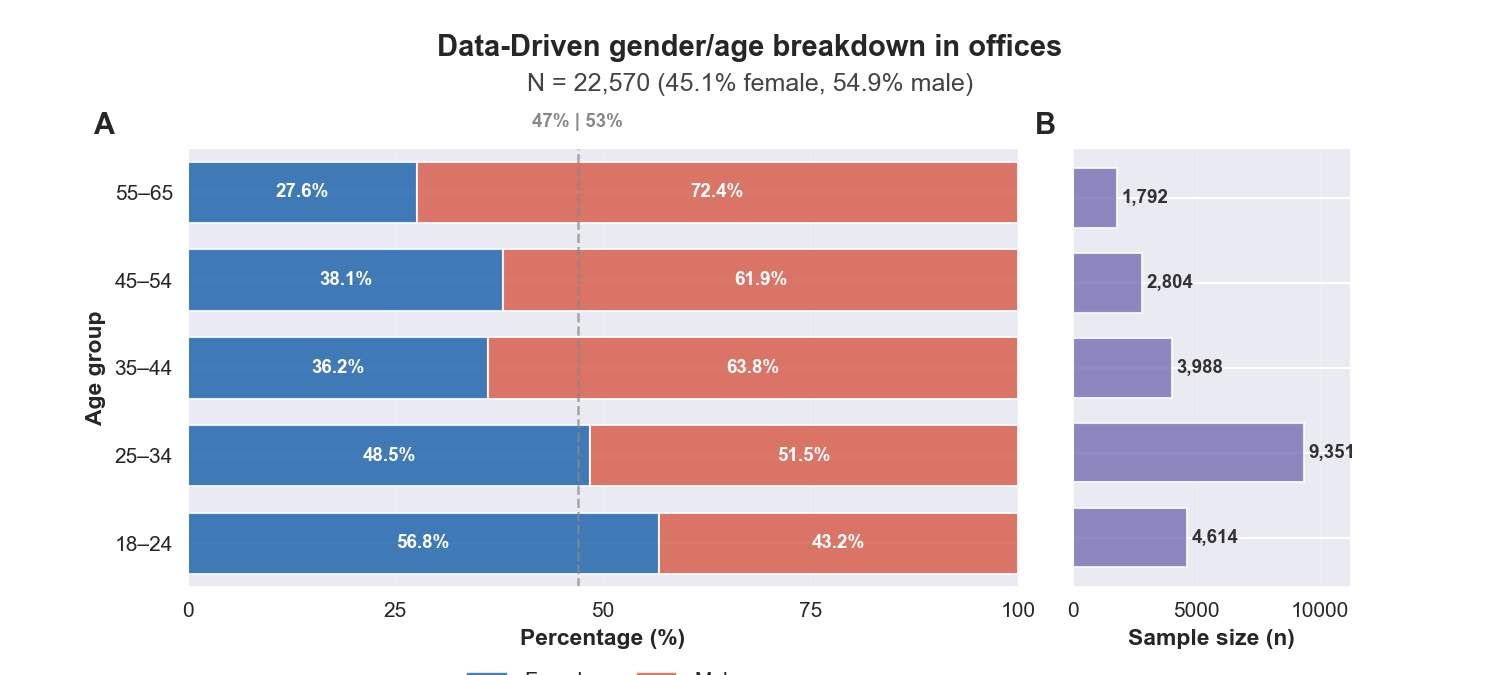
\includegraphics[width=0.75\linewidth]{figs/age_gen_breakdown.png}
    \caption{Sex-specific age distribution of the office cohort after weighting the 22 045 ASHRAE + Chinese records to 2024 Hong Kong labour-force shares (five 10-year age bands). Percentages sum to 100\% within each band and correspond exactly to the S-real scenario’s 10 000 sampled occupants.}
    \label{fig:age_sex}
\end{figure}

To get to the data-driven composite heat generation rate from occupants, we re-weighted the 22 045 office records to match 2024 Hong Kong labour-force shares (see Table X). Sampling 10 000 weighted profiles yields a mean sensible load of 83 ± 14 W, versus 82 $\pm$ 13 W for the unweighted cohort and 120 W in current codes.”

% ============================
% 2.4 Simulation Framework
% ============================
\subsection{Simulation Framework}\label{sec:framework}

\textbf{Climates.}  Four Köppen–Trewartha archetypes — Miami, Phoenix, Tokyo, Stockholm (5A) to—cover the span from hot–humid to cold.  
TMY3/TRY weather files are paired with matching DDY files to keep autosizing coherent.

\textbf{Solver.}  EnergyPlus 25.2 is executed via \textsc{Sinergym} with 15-min timesteps.  
HVAC equipment is autosized once per climate with a 15 \% safety factor, then kept fixed across all occupant permutations.

\textbf{Thermal Sensation Prediction.}  
Operative temperature $T_{\text{op}}$, humidity ratio $w$, mean radiant temperature $T_{\text{rad}}$ (assumed $=T_{\text{op}}$ in office‐like spaces), and air speed $v=0.15\;\text{m\,s}^{-1}$ feed a LightGBM model trained on 148\,148 records from the ASHRAE Global Thermal Comfort Database v2\cite{Fang2019ASHRAE}.  
The fitted mapping is

\begin{equation}
\widehat{\text{TSV}} = f_{\text{LGBM}}\!\left(T_{\text{op}},w,v,I_{\text{cl}},\dot{q}_{\text{met}}\right),
\end{equation}

with clothing insulation $I_{\text{cl}}=0.8\;\text{clo}$ for summer and $1.0\;\text{clo}$ for winter.  Five-fold cross-validation yields $\mathrm{RMSE}=0.47$ scale units.


Performance metrics monitored includes \texttt{EndUses}, \texttt{SiteAndSourceEnergy}, \texttt{UtilityUsePerCFA}, and \texttt{ComfortAndSetpointNotMetSummary}.  
Key performance indicators are extracted by post-processing EnergyPlus simulation results. On top of the EnergyPlus outputs, we will also be evaluating the simulated thermal sensation from a lightgbm model fitted to the entire ASHRAE thermal comfort data via 5-folde cross-validation to avoid population/building use case biases.
\dothis{Maybe write this with more arguments}

\[
    \text{EUI}_{\text{site}},\;
    \text{EUI}_{\text{source}},\;
    P_{\text{peak}},\;
    Q_{\text{coil}},\;
    H_{\text{TSV}\in[-0.5,0.5]},\;
    H_{\text{SetpointNotMet}}.
\]

Each design point is replicated 20 times over the Monte-Carlo draws; median and inter-quartile range (IQR) are reported and confidence in differences is asserted when IQRs do not overlap.

\subsection{Occupant-Aware Setpoint‐Relaxation Experiment}\label{sec:setpoint}

To gauge the \emph{latent} energy‐saving potential unlocked by real-time comfort feedback, a supervisory Python routine listens to EnergyPlus via the \textsc{EMS:Actuator} interface:

\begin{enumerate}
\item At each 15-min mark, i.e. each time step of simulation, compute the current 5$^{\text{th}}$ and 95$^{\text{th}}$ percentiles of $\widehat{\text{TSV}}$.
\item If the band lies inside $[-0.5,0.5]$, widen the active cooling and heating setpoints by  
      \[
        \Delta T = 0.5\;^{\circ}\text{C}\times\text{sgn}\!\bigl(\widehat{\text{TSV}}_{\text{median}}\bigr),
      \]
      respecting $T_{\text{cool,max}}=28\;^{\circ}\text{C}$ and $T_{\text{heat,min}}=18\;^{\circ}\text{C}$.
\item When the comfort band breaches $[-0.5,0.5]$, reset to the original fixed setpoints (24/22 °C cooling/heating).
\end{enumerate}

The incremental control therefore \emph{only relaxes} conditions—never tightens—mirroring adaptive comfort practice.  Energy impacts are summarised as

\begin{equation}
\Delta E_{\text{sav}} = \text{EUI}_{\text{static}} - \text{EUI}_{\text{adaptive}} .
\end{equation}

Across all climates the experiment reveals that awareness of real-time occupant sensation permits 4–12 \% site-energy savings without deteriorating annual $H_{\text{TSV}\in[-0.5,0.5]}$ (see §3.3).  

\paragraph{Scope Limitations.}
Internal gains from lighting and plug loads are held constant with density; window operation is excluded; and only a single VAV reheat system is considered.  These simplifications purposefully isolate metabolic‐rate effects and will be relaxed in future work.

